%This work is licensed under the Creative Commons Attribution-NonCommercial-NoDerivs 3.0 United States License. To view a copy of this license, visit http://creativecommons.org/licenses/by-nc-nd/3.0/us/ or send a letter to Creative Commons, 444 Castro Street, Suite 900, Mountain View, California, 94041, USA.

\section{Column Design and Construction}

Apart from the laser system, the majority of an Ultrafast Electron Microscope column is either vacuum hardware or contained within the vacuum system.
The vacuum chamber itself is almost entirely standard 4.5 in ConFlat (CF) hardware.
Much has been purchased from off-the-shelf hardware suppliers.
Some of the more specialized chamber components have been fabricated in-house or purchased from Kimball Physics Inc.

\begin{figure}
  \centering
  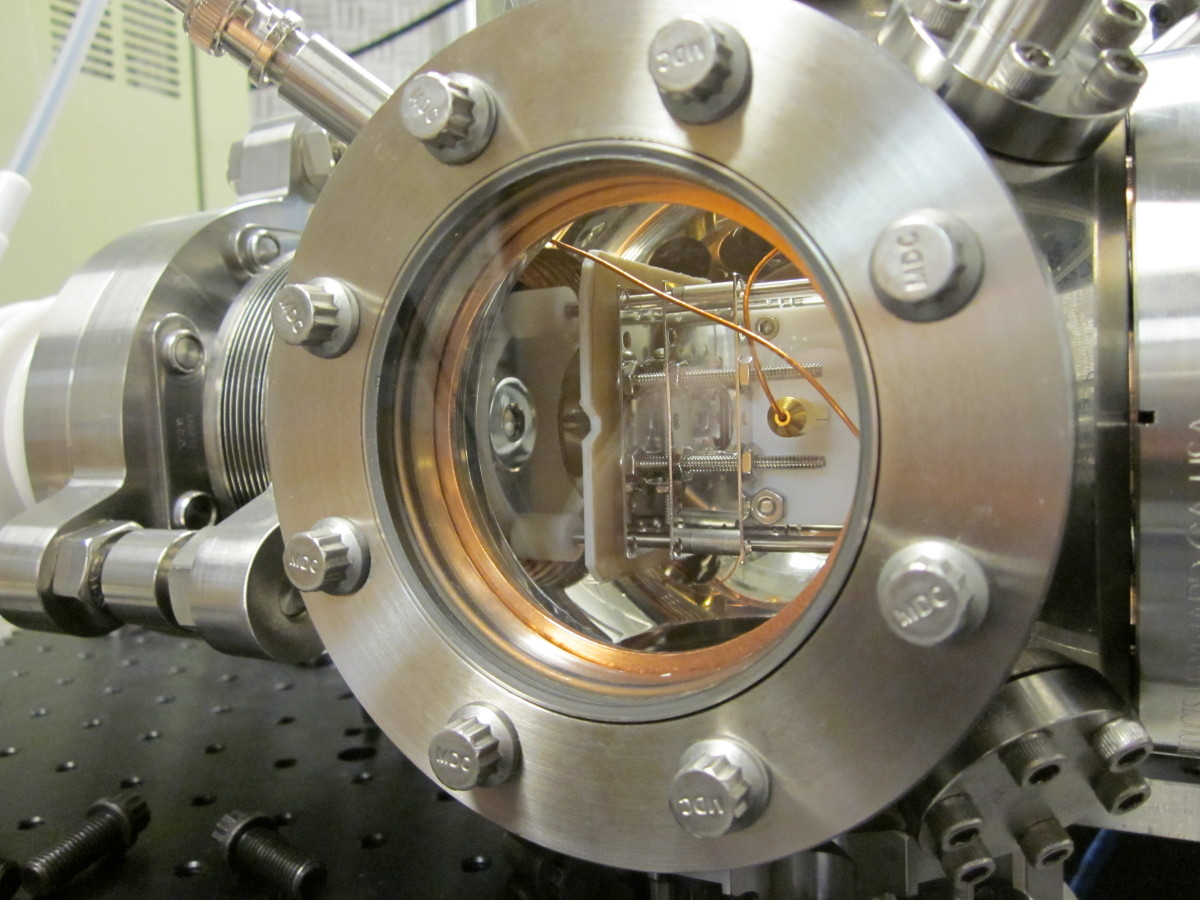
\includegraphics{chamber.jpg}
  \caption[Side view of main chamber]{
    Assembled side view of the main chamber section of the UEM column at UIC.
    To the left are the high-voltage passthrough and ``port aligner'' to which the cathode is mounted.
    Visible inside the window are the cathode Wehnelt and photocathode (left), the side of the anode, and the side of the deflector plates assembly just after the anode (right).
    The anode and plate-assembly are mounted by the ``eV Parts'' system attached to the main chamber.
    The wires and connectors supplying the voltage to the plates are also clearly visible.
  }
  \label{fig:chamber-pic}
\end{figure}

Kimball's line of Multi-CF hardware has been especially useful in building the prototype column.
The main chamber is a 4.5 in ``spherical cube''; a large stainless-steel sphere which has six 4.5 in ConFlat ports oriented as a cube, with another eight 1.33 in ports on the corners of the cube.
All ports on Multi-CF hardware also contain a set of grooves, designed as mounting points for a system of erector-set-like equipment called ``eV Parts.''
This system is used to mount the accelerator anode and the deflector plates which are both to be described later.


